\section{Background}\label{sec:background}

\subsection{TensorFlow Deep Learning Models}
\begin{figure}\centering
    \begin{subfigure}[b]{1\textwidth}
        \centering
        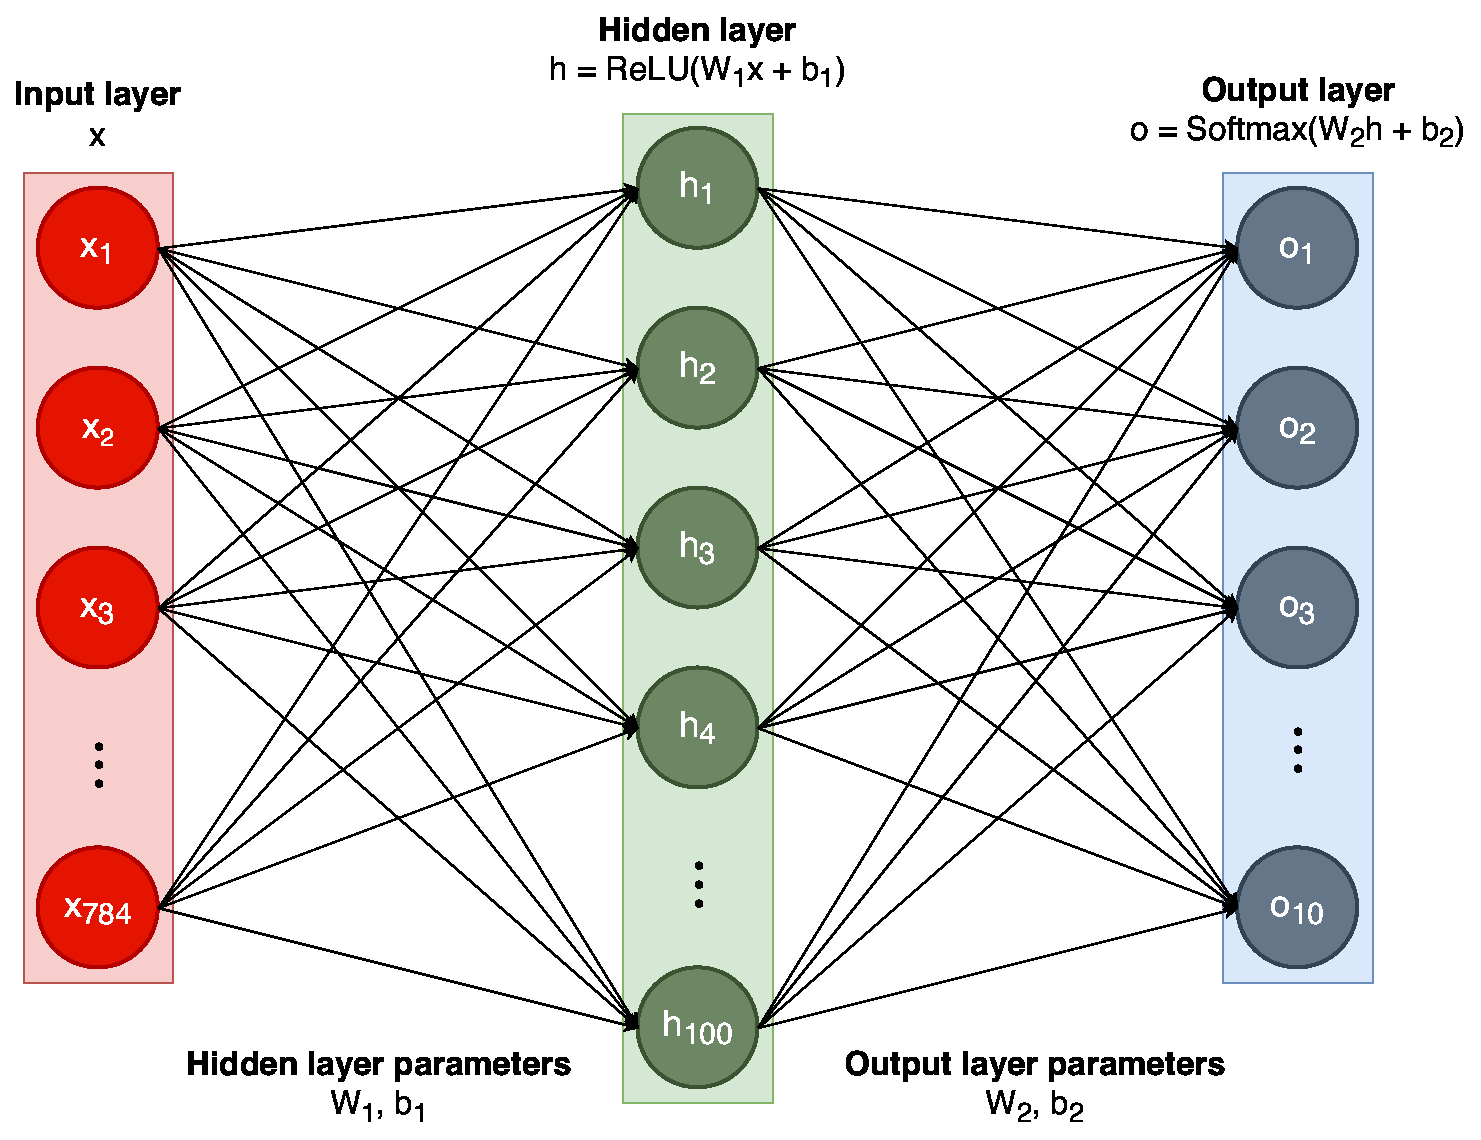
\includegraphics[width=0.7\textwidth]{Fig1.eps}
        \caption{The neural network with a hidden layer and an output layer}
        \label{fig:back:model}
    \end{subfigure}
    
    \begin{subfigure}[b]{1\textwidth}
        \lstinputlisting[style=mpython]{tensorflow1_mnist.py}
        \caption{TensorFlow 1.x model example}
        \label{fig:back:tf1}
    \end{subfigure}   
    \caption{An example neural network and TensorFlow 1.x model example}
    \label{fig:back:tf1_all}
\end{figure}

% \begin{figure}[ht!]\centering
% 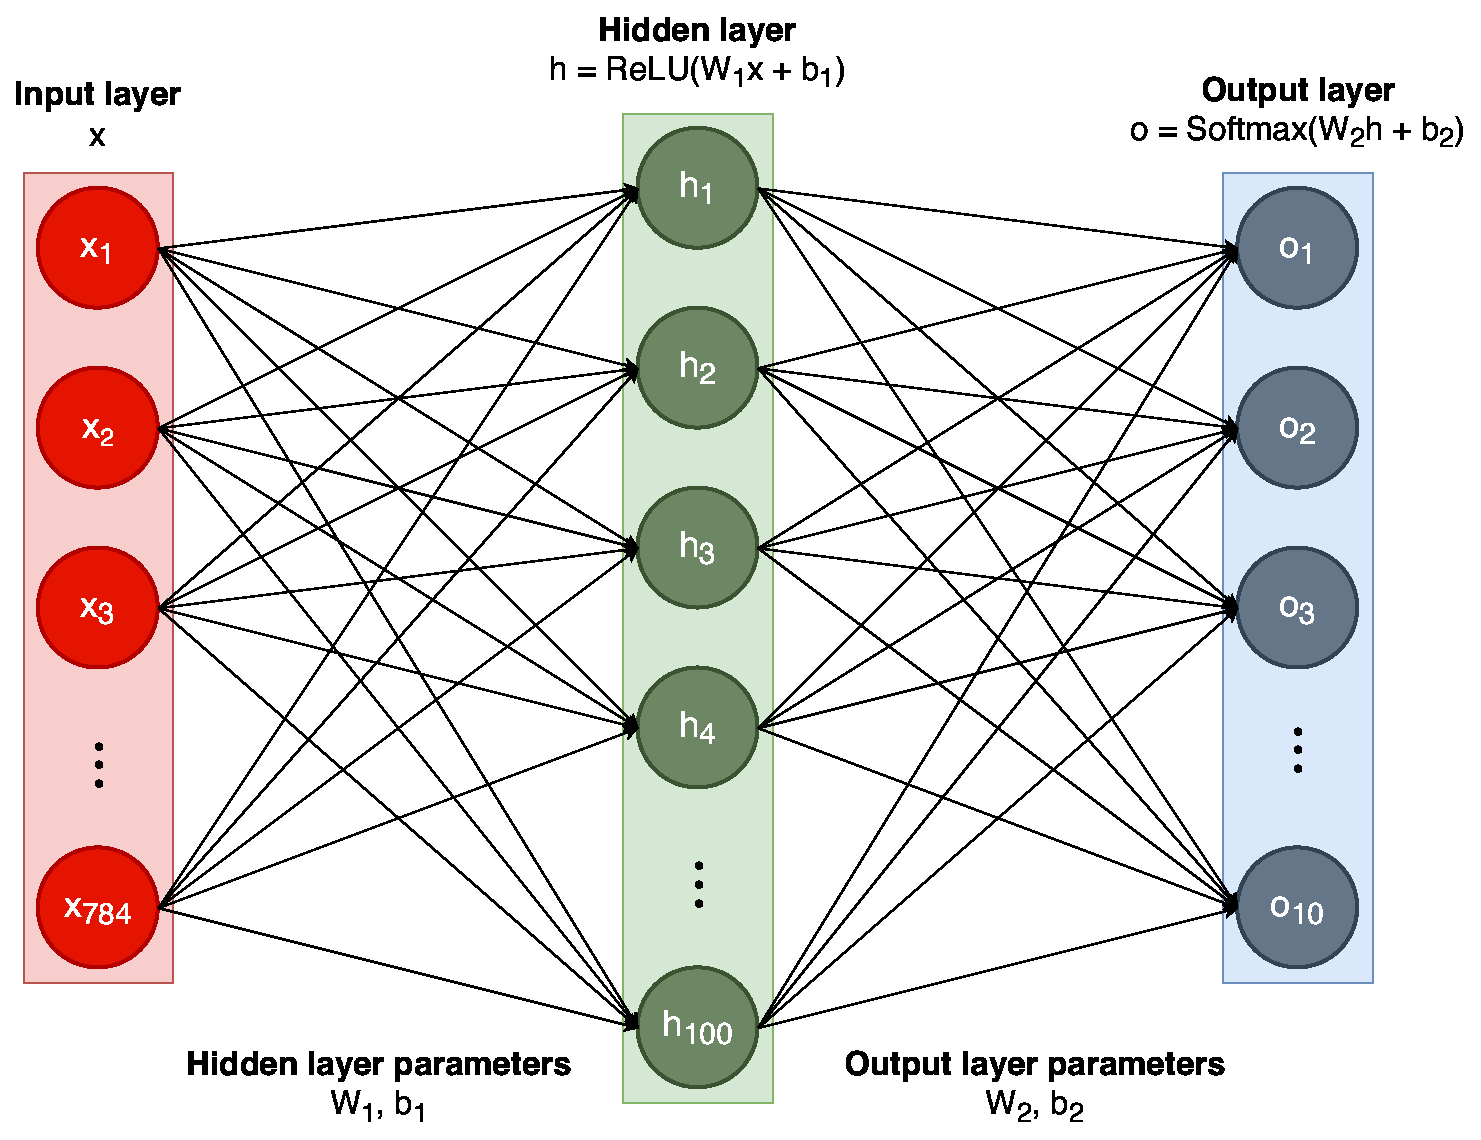
\includegraphics[width=1\textwidth]{Fig1.eps}
%   \caption{The neural network with a hidden layer and an output layer}
% \label{fig:back:model}
% \end{figure}

This section describes two different forms of TensorFlow DL models written in
Python.
TensorFlow provides two major version libraries: TensorFlow 1.x published in
2016 and TensorFlow 2.x published in 2019. 
DL models significantly differ in their forms depending on which library
they use. 
On TensorFlow 1.x, model engineers manually construct models as computational
graphs using tensor variables and operations and execute them lazily  for
training and inference on an encapsulated environment
called {\it session}.
%The first version is TensorFlow 1.x published in 2016.
%TensorFlow 1.x provides APIs for defining tensor variables and operations
%between them.
%Developers manually define the model structure, the model operations 
%and training process using the TensorFlow 1.x APIs.
%On TensorFlow 1.x, developers need to manually define model structures, model
%operations, and their training process using APIs for defining tensor variables
%and operations between them.
%The second version is TensorFlow 2.x published in 2019.
On the other hand, TensorFlow 2.x supports the eager execution that executes
all tensor operations as they occur in code. 
With the eager execution feature, engineers no longer need to construct
computational graphs and use encapsulated environments.
%developers to use plain Python syntax to define the model
%operations and the training process.
In addition, TensorFlow 2.x integrates with the Keras library, a layer-based
deep learning model library that provides a convenient interface to construct
models.
%As a result, the models written in TensorFlow 1.x and TensorFlow 2.x are
%significantly differ in their forms. 

Figure~\ref{fig:back:model} illustrates an example neural network that
classifies input images into ten categories.
% In the figure, vertical bars denote vectors of layers, circles denote data of
% vectors, and direct edges denote data dependencies from source to destination
% in vector operations.
%The model will get an input image of 784 pixels and classify it into one of ten
%output classes.
The network consists of three layers: an input, an output, and a hidden layer
between the two layers.
% Each layer stores data into a vector, and the vector of a layer mutates into a
% vector of another layer via vector operations.  
The input layer has a vector of length 784, and the data in the
vector is the pixels of an input image.
The hidden layer is parametrized by the two-dimensional weight matrix $W_1$ of
size 784 $\times$ 100 and the bias vector $b_1$ of length 100.
% The hidden layer's vector is computed by multiplying the input layer
% vector $x$ with the weight matrix $W_1$, adding the bias vector $b_1$, and
% finally applying the ReLU activation function that makes the results non-zero
% values.
The output layer is parametrized by the two-dimensional weight matrix $W_2$ of
size 100 $\times$ 10 and the bias vector $b_2$ of length 10.
% The output layer's vector is computed by multiplying the hidden
% layer vector $h$ with the weight matrix $W_2$, adding the bias vector $b_2$,
% and finally applying the Softmax activation function that converts the ten data
% to a probability distribution of the ten categories.
The weight matrices and the bias vectors in the network are model parameters,
and the training phase adjusts the model parameters repeatedly, to classify
input images correctly.
%The model structure is defined in terms of layers and operation between them.
%The layers are tensors of real values, which represent the signals and data.
%The model in the figure \ref{fig:back:model} has three layers;
%the input layer, the hidden layer, and the output layer.
%The layers are densely connected, which means that
%the layer outputs are computed by the linear transformation with 
%the weight matrices and the bias vectors, 
%and the non-linear activation functions. 
%The hidden layer is parametrized by the weight matrix
%$W_1$ of size (784, 100) and the bias vector $b_1$ of length 100.
%The hidden layer is computed by first multiplying the input layer vector $x$
%with the weight matrix $W_1$, adding the bias vector $b_1$, and finally applying
%the ReLU activation function to the result.
%The output layer is parametrized by the weight matrix $W_2$ of size (100, 10)
%and the bias vector $b_2$ of length 10.
%The output layer is computed by first multiplying the hidden layer vector $h$
%with the weight matrix $W_2$, adding the bias vector $b_2$, and finally applying
%the Softmax activation function to the result.
%The weight matrices and the bias vectors are called the model parameters 
%as their values are updated during the training process.
%The hidden layer is a vector of length 100.
%The output layer is a vector of length 10, and each vector element represents
%the probability of the input image classified into the corresponding class.

%We describe TensorFlow 1.x and 2.x versions with code examples that define
%the same model and the same training process.
%The code examples define the neural network model illustrated
%in the figure \ref{fig:back:model}.
%The model will get an input image of 784 pixels and classify it into one of ten
%output classes.
 
%The model structure is defined in terms of layers and operation between them.
%The layers are tensors of real values, which represent the signals and data.
%The model in the figure \ref{fig:back:model} has three layers;
%the input layer, the hidden layer, and the output layer.
%The input layer is a vector of length 784, which represents the input image
%of 784 pixels.
%The hidden layer is a vector of length 100.
%The output layer is a vector of length 10, and each vector element represents 
%the probability of the input image classified into the corresponding class.
%The layers are densely connected, which means that
%the layer outputs are computed by the linear transformation with 
%the weight matrices and the bias vectors, 
%and the non-linear activation functions. 
%The hidden layer is parametrized by the weight matrix
%$W_1$ of size (784, 100) and the bias vector $b_1$ of length 100.
%The hidden layer is computed by first multiplying the input layer vector $x$
%with the weight matrix $W_1$, adding the bias vector $b_1$, and finally applying
%the ReLU activation function to the result.
%The output layer is parametrized by the weight matrix $W_2$ of size (100, 10)
%and the bias vector $b_2$ of length 10.
%The output layer is computed by first multiplying the hidden layer vector $h$
%with the weight matrix $W_2$, adding the bias vector $b_2$, and finally applying
%the Softmax activation function to the result.
%The weight matrices and the bias vectors are called the model parameters 
%as their values are updated during the training process.

%The model is trained by the gradient descent algorithm. 
%The gradient descent algorithm is an iterative optimization algorithm
%that computes the gradients of model parameters to update their values toward
%local minimum of the loss function.
%The loss function defines the metric of the difference between the model 
%output and answer label.
%Thus, approaching the local minumum of the loss function means that the
%the gradient descent trains the model to return the output similar to the
%correct answer.
%In DL model training, the gradient descent is repeated against several
%training batches. Given a training input batch, the algorithm first computes
%the model loss with forward propagation then computes the gradients of the
%model parameters with backpropagation. The algorithm applies the gradients
%to update the model parameters, thus approaching to the minumum loss.

% \begin{figure}[ht!]\centering
% \lstinputlisting[style=mpython]
% {tensorflow1_mnist.py}
%   \caption{TensorFlow 1.x model example}
% \label{fig:back:tf1}
% \end{figure}

\begin{inred}
Figure~\ref{fig:back:tf1} is a training code written in TensorFlow 1.x.
\end{inred}
% Figure~\ref{fig:back:tf1} shows a TensorFlow 1.x model for the example neural
% network with the gradient descent training algorithm.
First, lines 5 to 14 define the network structure and the operations
between the layers.
% Lines 5 and 6 first create two placeholder variables, {\tt x} and {\tt y},
% where {\tt x} is a vector storing the pixel data of an input image, and {\tt y}
% is a vector storing the answer for the classification of the input image. 
% Lines 8 to 10 define the hidden layer.
% Line 8 creates a randomly initialized weight matrix {\tt W\_1}, and line 9
% creates a zero-initialized bias vector {\tt b\_1}.
% Then, the {\tt Variable} API wraps the matrix and the bias vector.
% The {\tt Variable} API creates a model parameter of which internal values are
% modifiable during training.
% Line 10 defines the operation of the hidden layer. It first multiplies the
% input vector {\tt x} with the weight matrix {\tt W\_1}, then adds the bias {\tt
% b\_1}, and finally applies the ReLU activation function. 
% Note that the line does not perform the operation but only defines how
% the input data mutates into the hidden layer's data while executing the
% model.
% Lines 12 to 14 define the output layer.
% Similar to lines 8 and 9, lines 12 and 13 define a randomly-initialized
% weight matrix {\tt W\_2}, and a zero-initialized bias vector {\tt b\_2}, as
% model parameters of the output layer.
% Then, line 14 defines the operation that
% multiplies the hidden layer output with
% the weight {\tt W\_2}, adds the bias vector {\tt b\_2}, and finally applies the
% {\tt softmax} activation function.
\begin{inred}
After constructing the neural network, the code defines the training algorithm
in lines 16 and 17.
Line 16 defines the categorical cross-entropy loss function,
and line 17 defines the Adam gradient descent algorithm~\cite{kingma2014adam}.
Lines 19 to 22 starts the main training loop
by creating a {\tt Session} object and repeatedly executing 
the training operation {\tt train\_op}.



\end{inred}


%As shown in the lines 5 to 14, developers must explicitly define
%the model components and oprations between them in TensorFlow 1.x model.

%Since the placeholder variables only specify the vector size of the input images
%and the labels; they will be replaced with actual values of the training
%data during the training process. 

%To define a neural network model in TensorFlow 1.x, 
%developers must explicitly define the model structure
%and the operations between the layers. 
%The developers also must manually start the training loop by explicitly
%accessing the TensorFlow runtime with dedicated APIs.

%The lines 8 to 10 defines the hidden layer.
%The line 8 uses the {\tt random\_uniform} API to create 
%a random weight matrix of size 784 by 100, 
%and the line 9 uses the {\tt zero} API to create a zero-vector of size 100.
%Then, the lines 8 and 9 wrap the weight matrix and the bias vector with
%{\tt Variable} API.
%The {\tt Variable} API creates a TensorFlow variable that can be later modified
%during the runtime. It is usually used to define a model 
%parameter, whose value is changed during the training process.
%Thus, the lines 8 and 9 create the weight and bias parameters for the
%hidden layer which have correct sizes and are modifiable during the 
%training process.
%The line 10 manually defines the operations of the hidden layer. 
%Note that the line does not actually compute the operations,
%but only define the operations that will be computed during the training.

% After constructing the neural network, the code defines the training algorithm
% in lines 16 and 17.
% Line 16 defines the categorical cross-entropy loss function that
% quantifies the degree of difference between the output data of {\tt layer\_2}
% and the answer {\tt y}.
% Line 17, then, creates an object of the {\tt AdamOptimizer} that is an
% implementation of the Adam gradient descent algorithm~\cite{kingma2014adam}.
% The {\tt minimize} method of the object generates a training operation that
% updates model parameters using the Adam gradient descent algorithm to minimize
% the loss calculated by the loss function.

%The lines 16 and 17 defines the loss function and the training operation. 
%The line 16 defines the loss function between the model output {\tt layer\_2} 
%and the answer label {\tt y} with categorial cross entropy function.
%The line 17 defines the training operation for the model.
%The line first calls the {\tt AdamOptimizer} constructor
%function to create an optimizer object.
%The optimizer objects in TensorFlow are abstractions of the gradient
%descent algorithms.
%For instance, the {\tt AdamOptimizer} abstracts a Adam gradient descent
%algorithm. % todo: cite Adam g.d.
%Then the {\tt minimize} method defines the training operation that updates the
%TensorFlow variables via the gradient descent on the first argument.
%Thus, the line 17 defines the operation of a single training step,
%which optimizes the model parameters via gradient descent to the loss gradient.

% Lines 19 to 22 train the model in a session.
% Line 19 creates a {\tt Session} object that provides an encapsulated
% environment storing model parameters.
% %that provides the {\tt run} method to execute the network's operations in an
% %encapsulated environment.
% %The line 20 calls the {\tt run} method with a global variable initializer
% %to initialize model parameters of the network.
% Line 20 calls the {\tt run} method of the object with a global variable
% initializer to initialize all the model parameters of the model in the
% encapsulated environment.
% %The {\tt Session} object provides the {\tt run} method that can invoke
% %computation of TensorFlow operations.
% %Before the training computation starts,
% %the TensorFlow variables in the model and the optimizer should be initialized.
% %Note that the optimizer object implicitly introduces the variables which are 
% %used for the internal computation.
% %After the variables are initialized, the line 21 uses the {\tt for} loop
% %to iterate over the dataset and get training input data. 
% Lines 21 and 22 then train the model in a loop that executes the training
% operation {\tt train\_op} with the input data {\tt x} and {\tt y} by iterating
% over the ten thousand input datasets obtained from {\tt dataset.take(10000)}.

%The number of training data is specified by the {\tt take} API of the
%dataset object.
%Finally, the line 22 calls the {\tt run} method to
%invoke computation of the training operation {\tt train\_op}.


\begin{figure}[ht!]
  \centering
  \begin{lstlisting}[style=mpython]
import tensorflow as tf

dataset = ...

model = tf.keras.Sequential([
    tf.keras.layers.Dense(100, activation='relu'),
    tf.keras.layers.Dense(10, activation='softmax')
])

loss = tf.losses.CategoricalCrossentropy()
opt = tf.optimizers.Adam(0.001)

for images, labels in dataset.take(10000):
    with tf.GradientTape() as tape:
        probs = model(images)
        loss_value = loss(labels, probs)

    grads = tape.gradient(loss_value, model.trainable_variables)
    opt.apply_gradients(zip(grads, model.trainable_variables)) \end{lstlisting}
  \caption{TensorFlow 2.x model example}
\label{fig:back:tf2}
\end{figure}

% new
In TensorFlow 2.x, engineers can more easily build DL models with the Keras
library and the eager execution feature.
Figure~\ref{fig:back:tf2} shows an implementation on TensorFlow 2.x for the
same model shown in Figure~\ref{fig:back:tf1}.
%Figure~\ref{fig:back:tf2} is a code example of TensorFlow 2.x model.
%The developers using TensorFlow 2.x define the model structure and the training
%loop. 
%The lines 5 to 8 define the model structure.
%First, the lines 5 to 8 use the Keras library APIs to define the neural network
%model with a hidden layer and an output layer.
Lines 5 to 8 construct the neural network as a sequential model from a
hidden layer to an output layer using the {\tt Sequential} API of the
library.
%Keras~\cite{keras} is a layer-based deep learning model library included in 
%TensorFlow 2.x. 
The {\tt Dense} API defines a layer by taking both the size of a vector and an
activation function. 
The API automatically creates a weight matrix and a bias vector of the layer
using the given size of a vector and the size of the vector of its previous
layer.
%The lines 6 and 7 define the dense layers with the {\tt Dense} API. 
%The first argument specifies the size of output vector.
%Given the output vector size, the {\tt Dense} API will automatically create
%the weight matrix and the bias vector parameters according to the size of 
%the previous layer. 
%The second argument of the {\tt Dense} API specifies the activation function of
%the layer, where the name of the activation function is given as a string. 
%The layers are then composed into a linear sequential model by the {\tt
%Sequential} API in the line 5.
%Compared to TensorFlow 1.x models, developers do not have to explicitly
%define the computation between the layers in TensorFlow 2.x.
Lines 10 and 11 define a loss function and an optimizer object.  
Unlike TensorFlow 1.x, TensorFlow 2.x provides APIs to select a loss function
used for the training, as shown in line 10.
Also, while TensorFlow 1.x explicitly defines a training operation of an
optimizer object and then executes it lazily on a session, TensorFlow 2.x
creates an optimizer object and later uses it to execute the
gradient descent algorithm eagerly during the training.
%The line 10 uses the {\tt CategoricalCrossentropy} API to 
%define the loss function.
%The line 11 uses the {\tt Adam} API to define the optimizer object.
%This optimizer object is equal to the {\tt AdamOptimizer} object in the 
%TensorFlow 1.x model.
%However, the usage of the optimizer object is different in two TensorFlow
%versions.
%In TensorFlow 1.x, the optimizer object is used to define the
%training operation {\tt train\_op}, which is later used as an argument
%for the {\tt Session.run} method to explicitly trigger the training step.
%In TensorFlow 2.x, the optimizer object is used to directly call the methods 
%that eagerly executes the gradient descent algorithm against the training input. 
Lines 13 to 19 train the model with a loop iterating over ten
thousand datasets.
Line 14 creates a {\tt GradientTape} object that records executed
operations for trainable model parameters within the {\tt with} scope.  
Lines 15 and 16 execute the model for an input image and calculate
the cross entropy loss between the execution output and the answer label. 
Because TensorFlow 2.x defines neural networks and loss functions as normal
Python functions, they can be called directly with arguments, as shown in the
lines.
%The training loop starts with the {\tt for} loop that iterates over the dataset
%and takes batches of training images and answer labels.
%Similar to the TensorFlow 1.x model,
%the line 13 uses the {\tt take} API to specify the number of batches.
%The line 14 creates a new {\tt GradientTape} object by {\tt with} statement.
%When a {\tt GradientTape} object is created by {\tt with} statement,
%it will record the gradients of the operations inside the {\tt with}
%statement body.
%The lines 15 and 16 define the forward propagation stage in a single
%training step.
%Note that in TensorFlow 2.x, the model object created with the Keras APIs can be
%used like a Python function as in the line 15.
%Thus, the line 15 computes the model output for the input training batch. 
%The line 16 computes the cross entropy loss between the model output and
%the answer label.
Lines 18 and 19 optimize the model parameters using the gradient descent
algorithm. 
The {\tt model.trainable\_variable} method returns the model parameters, and
the {\tt tape.gradient} method calculates the gradients using the recorded
operations on the model parameters and the loss value.
Then, line 19 optimizes the model parameters according to the
gradient descent algorithm by calling the {\tt apply\_gradients} method of the
optimizer object.

\subsection{Horovod Distributed Training Library}

Horovod~\cite{sergeev2018horovod} is a Python library for distributed training 
of TensorFlow models. 
The library adopts a model-parallel approach that creates one instance of a DL
model for each GPU.
%, leaving each GPU responsible for computing a single model instance
%computation.
%of distributed 
%training. 
%In model-parallel distributed training, multiple instances of the DL model
%are created, and each GPU takes responsibility of computing a single model
%instance computation. % <- todo: rephrase?
%Note that this means that the number of the model instances 
%is equal to the number of GPUs.
In the training phase, each GPU runs the computation of a single model instance
for a batch of input data and computes a loss separately.
The library updates the model parameters using the gradient descent algorithm
with gradients computed from the average loss of the instances.
Thus, engineers can take advantage of parallelism to train DL models in a
shorter time on multiple GPUs.
%Thus, developers can take advantage of parallelism by separate input data into
%{\it N}-batches and train a DL model for each batch on each GPU
%parallely.shorter time on multiple GPUs.
%In training process, each model instance gets a training batch and computes the
%loss value. 
%Then the loss gradients are averaged across the GPUs to synchronize the model
%states. 
%The gradient descent algorithm updates the model parameters by the averaged
%gradients.
%By the model-parallel distributed training, developers can take advantage of
%parallelism to train their DL model in shorter time.

\begin{figure}[ht!]
  \begin{lstlisting}[style=mpython]
import tensorflow.compat.v1 as tf
import horovod.tensorflow as hvd

hvd.init()
config = tf.ConfigProto()
config.gpu_options.allow_growth = True
config.gpu_options.visible_device_list = str(hvd.local_rank())

dataset = ...

x = tf.placeholder(tf.float32, [BATCH_SIZE, 784])
y = tf.placeholder(tf.float32, [BATCH_SIZE, 10]) 

W_1 = tf.Variable(tf.random_uniform([784, 100]))
b_1 = tf.Variable(tf.zeros([100]))
layer_1 = tf.nn.relu(tf.matmul(x, W_1) + b_1)

W_2 = tf.Variable(tf.random_uniform([100, 10]))
b_2 = tf.Variable(tf.zeros([10]))
layer_2 = tf.nn.softmax(tf.matmul(layer_1, W_2) + b_2)

loss = -tf.reduce_sum(y * tf.log(layer_2), 1) # Categorical cross entropy 
train_op = hvd.DistributedOptimizer(tf.train.AdamOptimizer(0.001 * hvd.size())).minimize(loss)

with tf.Session() as sess:
  sess.run(tf.global_variables_initializer())
  sess.run(hvd.broadcast_global_variables(root_rank=0))
  for images, labels in dataset.take(10000 // hvd.size()): 
    sess.run(train_op, {x: images, y: labels}) \end{lstlisting}
  \caption{Horovod distributed model example for TensorFlow 1.x model}
\label{fig:back:hvd1} 
\end{figure}

Horovod requires model engineers to rewrite TensorFlow DL models with the
Horovod API for distributed training.
Figure~\ref{fig:back:hvd1} represents a distributed model rewritten from the
TensorFlow 1.x model example in Figure~\ref{fig:back:tf1}.
The distributed model has four big differences from the single-GPU model.
1) It configures GPUs and processes for distributed training.
Line 4 initializes the Horovod configuration by calling {\tt hvd.init()},
and lines 5 to 7 create the same number of processes with GPUs in the
system and pin each GPU per process. 
The GPU pinning ensures that each model instance trains on a single
dedicated GPU.
2) The distributed model uses the distributed version of the gradient
descent algorithm. 
Line 23 creates the same optimizer {\tt tf.train.AdamOptimizer} with the
learning rate multiplied by the number of GPUs, {\tt hvd.size()}. 
According to the Horovod library document, the learning rate of the distributed
optimizer should be scaled by the number of GPUs for efficient distributed
training. 
Moreover, line 23 wraps the optimizer with the {\tt DistributedOptimizer}
API. 
The API takes a single GPU-based optimizer and produces its distributed version
that averages the loss gradients across the training processes.
3) The distributed model synchronizes the model's and the optimizer's variables
across the training processes.
According to the Horovod library document, variables should be synchronized
exactly once after initializing the variables.
Therefore, line 27 broadcasts the variables across the training processes
via {\tt broadcast\_global\_variables} API.
4) The distributed model divides input data into multiple batches of the same
number as the training processes. 
Lines 28 and 29 run multiple training processes simultaneously, on which
each model instance gets trained with one of the batches obtained from {\tt
dataset.take(10000 // hvd.size())}. 
%The variable broadcasting is a process where the TensorFlow 
%variable values in different training processes are synchronized into
%the same value.
%In figure \ref{fig:back:hvd1}, the variable broadcasting is done in the line 27,
%which is right after the line 26 that initializes the TensorFlow variables,
%and right before the line 28 that starts the training loop.
%Note that the {\tt broadcast\_global\_variables} API broadcasts every
%TensorFlow variables including the model variables and the optimizer
%variables.


%The line 23 defines the training operation, 
%which is a distributed version of the gradient descent algorithm.
%Compared to the line 17 in the figure~\ref{fig:back:tf1},
%the line 23 makes two changes to the optimizer object.
%First, the learning rate argument is multiplied by {\tt hvd.size()}.
%According to the Horovod library document,
%the learning rate of the distributed optimizer 
%should be scaled by the number of GPUs for efficient distributed training.
%To acheive this, the line 23 calls the {\tt hvd.size()} method to
%get the total number of processes that Horovod has created,
%which is equal to the number of GPUs.
%Second, the optimizer object is wrapped with the Horovod library API,
%{\tt DistributedOptimizer}.
%The {\tt DistributedOptimizer} API converts the single GPU-based optimizer 
%object to distributed optimizer, which averages the loss gradients across the
%training processes.
%Thus, wrapping the optimizer with {\tt DistributedOptimizer} API is necessary
%for correct distributed training of the model.

%To explain how to rewrite single-GPU TensorFlow models into the distributed 
%models with Horovod library, we provide the code examples of distributing 
%the TensorFlow 1.x model in the figure~\ref{fig:back:tf1} and the TensorFlow
%2.x model in the figure~\ref{fig:back:tf2}.

%To explain how to rewrite single-GPU TensorFlow models into the distributed 
%models with Horovod library, we provide the code examples of distributing 
%the TensorFlow 1.x model in the figure~\ref{fig:back:tf1} and the TensorFlow
%2.x model in the figure~\ref{fig:back:tf2}.
%We focus on explaining the difference between the original model codes in
%the figures~\ref{fig:back:tf1}, \ref{fig:back:tf2} and the distributed 
%model codes in the following paragraphs.

%todo: paragraph 나누는 기준 좀 고민
% p1 : figure intro, explain initialization + gpu pinning

%Figure~\ref{fig:back:hvd1} is a code example of using Horovod to distribute
%the TensorFlow 1.x model in~\ref{fig:back:tf1}.
%The line 4 first initializes the Horovod configuration.
%The lines 5 to 7 create the same number of processes with GPUs in the system,
%and pins each GPU per process. 
%The GPU pinning is a process where each GPU in the system is assigned to a 
%single training process.
%This is done by refering to the local rank of the process 
%by the {\tt local\_rank} API.
%This ensures that each model instance is trained by a single dedicated GPU.

% p2: explain optimizer
%The line 23 defines the training operation, 
%which is a distributed version of the gradient descent algorithm.
%Compared to the line 17 in the figure~\ref{fig:back:tf1},
%the line 23 makes two changes to the optimizer object.
%First, the learning rate argument is multiplied by {\tt hvd.size()}.
%According to the Horovod library document,
%the learning rate of the distributed optimizer 
%should be scaled by the number of GPUs for efficient distributed training.
%To acheive this, the line 23 calls the {\tt hvd.size()} method to
%get the total number of processes that Horovod has created,
%which is equal to the number of GPUs.
%Second, the optimizer object is wrapped with the Horovod library API,
%{\tt DistributedOptimizer}.
%The {\tt DistributedOptimizer} API converts the single GPU-based optimizer 
%object to distributed optimizer, which averages the loss gradients across the
%training processes.
%Thus, wrapping the optimizer with {\tt DistributedOptimizer} API is necessary
%for correct distributed training of the model.

% p3: explain variable broadcast
%The line 27 broadcasts the model and optimizer variables across the training
%processes.
%The variable broadcasting is a process where the TensorFlow 
%variable values in different training processes are synchronized into
%the same value.
%According to the Horovod library document, the variable broadcasting
%should occur exactly once during the training process,
%right after the variables are initialized.
%In figure \ref{fig:back:hvd1}, the variable broadcasting is done in the line 27,
%which is right after the line 26 that initializes the TensorFlow variables,
%and right before the line 28 that starts the training loop.
%Note that the {\tt broadcast\_global\_variables} API broadcasts every
%TensorFlow variables including the model variables and the optimizer
%variables.

% p4 : dataset length scale
%Finally, the line 28 starts the training loop.
%According to the Horovod library document, the number of training data
%batches can be scaled down by the number of GPUs as the same number of
%the batches are simultaneously trained in one training step.
%Thus, the line 29 divides the number of batches taken from the dataset
%by the number of the GPUs, {\tt hvd.size()}.


\begin{figure}[ht!]
  \begin{lstlisting}[style=mpython]
import tensorflow as tf
import horovod.tensorflow as hvd

hvd_broadcast_done = False
hvd.init()

gpus = tf.config.experimental.list_physical_devices('GPU')
for gpu in gpus:
    tf.config.experimental.set_memory_growth(gpu, True)
if gpus:
    tf.config.experimental.set_visible_devices(gpus[hvd.local_rank()], 'GPU')

model = tf.keras.Sequential([
    tf.keras.layers.Dense(100, activation='relu'),
    tf.keras.layers.Dense(10, activation='softmax')
])

loss = tf.losses.CategoricalCrossentropy()
opt = tf.optimizers.Adam(0.001 * hvd.size())

for images, labels in dataset.take(10000 // hvd.size()):
    with tf.GradientTape() as tape:
        probs = model(images)
        loss_value = loss(labels, probs)    

    tape = hvd.DistributedGradientTape(tape)

    grads = tape.gradient(loss_value, model.trainable_variables)
    opt.apply_gradients(zip(grads, model.trainable_variables))

    if not hvd_broadcast_done:
        hvd.broadcast_variables(model.variables, root_rank=0)
        hvd.broadcast_variables(opt.variables(), root_rank=0)
        hvd_broadcast_done = True  \end{lstlisting}
  \caption{Horovod distributed model example for TensorFlow 2.x model}
\label{fig:back:hvd2} 
\end{figure}

% todo: detailed expl of gpu pinning also for 1.x?
% todo : detailed xpl of "memory growth" for gpu pininng
% p1: init & gpu pinning
Because TensorFlow 2.x models differ from TensorFlow 1.x, Horovod
suggests different ways to rewrite models depending on the TensorFlow version.
Figure~\ref{fig:back:hvd2} is a distributed model rewritten from the
TensorFlow 2.x model example in Figure~\ref{fig:back:tf2}.
Lines 4 and 5 initialize the Horovod configuration and a boolean flag
{\tt hvd\_broadcast\_done} set to {\tt False}.
Lines 7 to 11 get the list of GPUs in the system and pin each GPU per
process. 
While TensorFlow 1.x uses {\tt ConfigProto()} for the configuration, the lines
use {\tt config.experimental} instead since {\tt ConfigProto()} is deprecated
in TensorFlow 2.x.
%The line 7 first gets the list of GPUs in the system.
%The line 11 pin the GPU to the process, using the local rank of the process.
% p2 : optimizer lr
Line 19 defines the optimizer object with the learning rate multiplied by
the number of GPUs but without wrapping {\tt DistributedOptimizer}.
%As in the optimizer of figure \ref{fig:back:hvd1}, 
%the learning rate argument of the optimizer object 
%should be scaled by {\tt hvd.size()} for efficient distributed training. 
% p3 : dataset length
Line 21 starts the training loop for each model instance with a batch of
input data obtained from {\tt dataset.take(10000 // hvd.size())}.
%As mentioned before, the number of training data batches can be
%scaled down by the number of GPUs.
%To implement this, the {\tt for} loop in the line 21
%divides the number of batches taken from the dataset by {\tt hvd.size()}.
% p4 : tape
Inside the training loop,
line 26 wraps the {\tt GradientTape} object with the Horovod API  {\tt
DistributedGradientTape}.
The {\tt DistributedGradientTape} averages the loss gradients across the
training processes like the {\tt DistributedOptimizer} in the
distributed TensorFlow 1.x model.
%API is similar
%to the {\tt DistributedOptimizer} API in distributed TensorFlow 1.x model; 
%the loss gradients will be averaged across the training processes 
%before the gradient descent.
%Thus, wrapping the {\tt GradientTape} object with the 
%{\tt DistributedGradientTape} API is necessary for correct training
%of the model.
% p5. broadcast
Finally, lines 31 to 34 broadcast the model and optimizer variables
across the training processes.
%As mentioned before, the variable broadcasting should occur exactly once,
%right after the variables are initialized.
%To ensure the variable broadcasting occur only during the first training step,
%the line 31 uses the global boolean variable {\tt hvd\_broadcast\_done},
%then changes the value in the line 34 after the broadcasting is done.
%Also note that the broadcasting code is placed right after the line 29,
%where the optimizer method {\tt apply\_gradient} is finished.
%In TensorFlow 2.x, the variables are not explicitly initialized,
%but rather implicitly initialized during the first computation involving the
%variable.
TensorFlow 2.x implicitly initializes variables once when applying the
optimizer's {\tt apply\_gradients} function to {\tt
model.trainable\_variables}.
Thus, after applying the function, the code calls the {\tt
hvd.broadcast\_variables} API to broadcast the variables and sets the boolean
flag {\tt hvd\_broadcast\_done} to {\tt True} to prevent repeated broadcasting.
%To ensure that the variable broadcasting happen after the optimizer
%variables are initialized, the variable broadcasting codes are placed
%after the first gradient descent step is finished, thus the optimizer
%variables are already initialized.
